\documentclass[12pt]{article}

\usepackage{sbc-template}
\usepackage{graphicx,url}
\usepackage{booktabs}
\usepackage[utf8]{inputenc}
\usepackage[brazil]{babel}

\sloppy

\title{Mineração de Métricas DORA em Repositórios Open Source: \\ Quanto Podemos Confiar nos Proxies?}

\author{Gabriel Chagas\inst{1}, Guilherme Lana\inst{1}, Marcus Vinicius\inst{1}}

\address{Pontifícia Universidade Católica de Minas Gerais (PUC Minas) -- Engenharia de Software\\
  Belo Horizonte -- MG -- Brasil
  \email{gabrielchlage@gmail.com, contato.guilhermelana@gmail.com, marcus.alves.1436506@pucminas.com.br}
}

\begin{document}

\maketitle

\begin{abstract}
  We mined the four DORA delivery metrics from 300 popular open-source GitHub
  repositories that use GitHub Actions, over a 12-month window. Since GitHub
  records neither deployments nor production failures, every metric is a proxy.
  The proxies disagree: the median change failure rate is 4.9\% when measured
  by CI runs and 23.5\% when measured by releases followed by a corrective
  release. Changing the operational definitions moves 34.3\% of the repositories
  to another DORA category, almost entirely because of the failure rate. Deploy
  frequency correlates positively with failure rate ($\rho$ = 0.18 and 0.62),
  and repository age is the factor most associated with performance. A manual
  gold sample showed that ``corrective release'' is ambiguous (Fleiss
  $\kappa$ = 0.32).
\end{abstract}

\begin{resumo}
  Minerou-se as quatro métricas DORA de 300 repositórios open source populares
  do GitHub que usam GitHub Actions, numa janela de 12 meses. Como o GitHub não
  registra deploys nem falhas em produção, toda métrica é um proxy, e os proxies
  discordam: a mediana da taxa de falha é 4,9\% medida pelo CI e 23,5\% medida
  por releases seguidas de uma release corretiva. Trocar as definições
  operacionais muda a categoria DORA de 34,3\% dos repositórios, quase só por
  causa da taxa de falha. A frequência de deploy tem correlação positiva com a
  taxa de falha ($\rho$ = 0,18 e 0,62), e a idade do repositório é o fator mais
  associado ao desempenho. A validação manual mostrou que ``release corretiva''
  é um critério ambíguo (kappa de Fleiss = 0,32).
\end{resumo}

\section{Introdução}

As métricas DORA (\emph{DevOps Research and Assessment}) tornaram-se o padrão
de mercado para medir o desempenho de entrega de software
\cite{forsgren:2018,dora:guide}. São quatro: frequência de deploy (\emph{deployment
frequency}), tempo entre o commit e a produção (\emph{lead time for changes}),
proporção de deploys que causam falha (\emph{change failure rate}, CFR) e
tempo de recuperação de um deploy que falhou. As duas primeiras medem
velocidade, e as duas últimas, estabilidade.

O GitHub, porém, \textbf{não registra deploys em produção nem falhas em
produção}. Um projeto open source publica \emph{releases}, executa
\emph{workflows} de CI e recebe commits, e é a partir disso que as métricas
precisam ser \emph{inferidas}. Uma medida indireta como essa é um \emph{proxy}:
``release publicada'' faz as vezes de deploy, e ``execução de CI que falhou''
faz as vezes de falha. Proxies podem enganar. Por isso este trabalho faz duas
perguntas: qual é o valor de cada métrica em repositórios populares e, também,
\emph{quanto podemos confiar nesse valor}.

Respondemos a sete questões de pesquisa (RQ) e a uma bônus, sobre 300
repositórios:
\textbf{RQ1}~frequência de deploy;
\textbf{RQ2}~lead time (por release e por commit);
\textbf{RQ3}~taxa de falha (proxy de CI e proxy de entrega);
\textbf{RQ4}~tempo de recuperação;
\textbf{RQ5}~relação entre frequência de deploy e taxa de falha;
\textbf{RQ6}~características dos repositórios associadas ao desempenho;
\textbf{RQ7}~sensibilidade da classificação DORA à definição operacional;
e \textbf{RQ8}~(bônus) \emph{rework rate}.

\textbf{Hipóteses informais.} O que o grupo espera encontrar em cada questão,
derivado do referencial DORA e das definições operacionais adotadas (versão
completa em \texttt{docs/hipoteses.md}).

\textbf{RQ1:} mediana bem abaixo do corte Elite, entre uma release por mês e
uma por semana --- publicar release é evento de empacotamento, não de deploy
contínuo. \textbf{RQ2:} a variante (a) deve ser sistematicamente maior que a
(b), porque usa o commit mais antigo da release, que é um máximo sensível a um
único commit esquecido. \textbf{RQ3:} o proxy de CI deve dar valores baixos e o
de entrega valores bem maiores, e as duas variantes devem discordar; esperamos
que o sinal de \emph{patch} sozinho tenha recall alto e precisão baixa, e que
seja preciso combinar sinais para atingir F1 $\ge$ 0,70. \textbf{RQ4:} medianas
na casa de horas e pouca censura, porque CI quebrado no branch principal
bloqueia todo mundo. \textbf{RQ5:} não esperamos o \emph{trade-off} clássico,
mas também não leremos correlação positiva como evidência a favor do DORA: o
CFR (b) exige uma release seguinte em até 7 dias, e quem publica mais tem mais
chance de tê-la, o que produziria correlação por mecânica da definição.
\textbf{RQ6:} efeitos pequenos e poucos sobreviventes à correção de Holm;
apostamos em tipo de projeto e número de contribuidores acima de popularidade,
porque estrelas medem visibilidade e não prática de engenharia. \textbf{RQ7:}
parcela substancial dos repositórios deve mudar de categoria, com o CFR movendo
mais que o lead time. \textbf{RQ8:} a \emph{rework rate} deve ser maior que o
CFR (b), por contar correções de qualquer prazo, e deve correlacionar menos com
a frequência de releases.

\section{Metodologia}

\subsection{Coleta e seleção}

Os dados vêm exclusivamente da API REST do GitHub, acessada por um cliente
próprio, sem bibliotecas de terceiros. Toda resposta é guardada em disco, de
modo que a coleta pode ser interrompida e retomada sem repetir chamadas. O
cliente respeita a cota por hora e a proteção contra rajadas, e repete erros
temporários com \emph{backoff} exponencial. Por repositório, coletamos
metadados, \emph{workflow runs} do \emph{default branch} disparados por
\texttt{push}, releases não-rascunho e os commits entre releases consecutivas
(obtidos por clone local, sem o teto de commits do \texttt{compare}).

Os candidatos vêm de buscas por faixa de estrelas (de 1.000 a mais de 50.000),
porque a API limita cada busca a 1.000 resultados. A lista é ordenada,
embaralhada com semente fixa (42) e avaliada até completar 300 repositórios. A
Tabela~\ref{tab:funil} mostra o funil: exigimos pelo menos 5 releases e 50
workflow runs válidos na janela de observação, de 1/10/2025 a 30/09/2026.

\begin{table}[ht]
\centering
\caption{Funil de seleção dos repositórios}
\label{tab:funil}
\small
\begin{tabular}{lrr}
\toprule
Etapa & Restantes & Descartados \\
\midrule
Candidatos (busca por faixas de estrelas) & 4.511 & -- \\
Forks ou arquivados & 4.407 & 104 \\
Sem push na janela & 4.092 & 315 \\
Sem GitHub Actions & 3.985 & 107 \\
Menos de 5 releases na janela & 3.559 & 426 \\
Menos de 50 runs válidos na janela & 3.492 & 67 \\
Amostra final (sorteio, semente 42) & 300 & 3.192 (não avaliados) \\
\bottomrule
\end{tabular}
\end{table}

\subsection{Definições operacionais}

A Tabela~\ref{tab:def} resume as métricas e suas variantes. Deploy é uma
\emph{release publicada} que não é rascunho nem pré-release, e a data de um
commit é a \texttt{author\_date}. Para o CFR (a), falha é \texttt{failure},
\texttt{timed\_out} ou \texttt{startup\_failure}, e execuções canceladas ou
puladas são ignoradas. No CFR (b), uma release \emph{falhou} se foi seguida,
em até 7 dias, por uma release corretiva. As publicadas nos últimos 7 dias da
janela ficam fora do denominador (censura). No tempo de recuperação, os
episódios de falha são calculados \emph{dentro} de cada workflow, e os que não
terminam na janela são censurados, não descartados. Em todas as métricas, o
valor do repositório é a \textbf{mediana}, e as tabelas reportam mediana e
intervalo interquartil (IQR), porque as distribuições são muito assimétricas.

\begin{table}[ht]
\centering
\caption{Métricas e variantes}
\label{tab:def}
\small
\begin{tabular}{p{2.3cm}p{9.7cm}}
\toprule
Métrica & Definição operacional \\
\midrule
Frequência & Releases publicadas na janela $\div$ semanas da janela \\
Lead time (a) & Por release: publicação $-$ commit mais antigo que ela entrega \\
Lead time (b) & Por commit: publicação $-$ data de cada commit novo \\
CFR (a) & Falhas $\div$ (falhas + sucessos) dos runs de push no \emph{default branch} \\
CFR (b) & Releases seguidas, em até 7 dias, por uma corretiva $\div$ releases avaliadas \\
Recuperação & Sucesso seguinte $-$ primeira falha, por workflow \\
\bottomrule
\end{tabular}
\end{table}

A classificação DORA usa os cortes fixos da disciplina (Elite, High, Medium e
Low) em cada métrica. A categoria geral é a mediana das quatro notas (4 a 1),
arredondada para baixo.

\subsection{Validação manual e heurística corretiva}

Não há campo na API que marque uma release como corretiva. Usamos uma
heurística sobre três sinais: o número de \emph{patch} do versionamento
semântico \cite{semver} é maior que zero; a tag ou o título cita
\emph{fix}, \emph{hotfix}, \emph{bugfix} ou \emph{revert}; ao menos metade dos
commits novos cita essas palavras. As versões v1 a v4 combinam esses sinais
(v1: \emph{patch}; v2: \emph{patch} ou nome; v3: commits; v4: qualquer um).

Para medir o erro, sorteamos 60 repositórios (semente 42) e, em cada um, até 5
releases (300 no total). Os três autores rotularam a amostra de forma
independente, sem consultar os colegas e sem ver a saída da heurística, em três
dimensões: tipo do projeto, se as releases são entregas reais e se cada release
é corretiva. A concordância foi medida pelo kappa de Fleiss e interpretada
pela escala de Landis e Koch \cite{landis:1977}. O consenso é a maioria
simples, e a heurística é avaliada contra ele por precisão, recall e F1, com
meta de F1 $\ge$ 0,70.

\subsection{Análise estatística}

RQ5 usa a correlação de Spearman ($\rho$). RQ6 compara as métricas entre
subgrupos com Kruskal-Wallis (ou Mann-Whitney, com dois grupos), com correção
de Holm para comparações múltiplas e tamanhos de efeito $\varepsilon^2 = H/(n-1)$
e $\delta$ de Cliff \cite{romano:2006}. Os fatores são linguagem, estrelas,
contribuidores e idade (os três últimos em quartis). RQ7 compara cinco
combinações de definições (C1 a C5) pelo kappa de Cohen ponderado linearmente,
com IC de 95\% por \emph{bootstrap} dos repositórios.

\subsection{Reprodutibilidade}

A coleta roda com um único comando, o token do GitHub é lido de uma variável de
ambiente, as sementes estão fixas e há testes automatizados executados no CI do
repositório\footnote{\url{https://github.com/gabrielchagas13/lab-exp-de-software-turma-02-grupo-06}}.
Os dados brutos são versionados em Parquet, e cada coluna dos CSVs finais está
documentada em um dicionário de dados.

\section{Resultados}

\subsection{RQ1 a RQ4: as quatro métricas}

\begin{table}[ht]
\centering
\caption{Mediana e IQR por repositório (300 repositórios)}
\label{tab:desc}
\small
\begin{tabular}{lrr}
\toprule
Métrica & Mediana & IQR \\
\midrule
Releases por semana (RQ1) & 0,44 & 0,23 -- 1,04 \\
Lead time (a), horas (RQ2) & 226,3 & 68,1 -- 818,0 \\
Lead time (b), horas (RQ2) & 179,8 & 52,4 -- 900,9 \\
CFR (a), proxy de CI (RQ3) & 4,9\% & 2,1 -- 10,9\% \\
CFR (b), v5 \emph{patch} e notas (RQ3) & 23,5\% & 0,0 -- 49,4\% \\
CFR (b), v2 semver ou nome (RQ3) & 37,5\% & 12,5 -- 64,1\% \\
CFR (b), v3 commits (RQ3) & 10,8\% & 0,0 -- 31,6\% \\
Recuperação, horas (RQ4; 276 repos) & 2,70 & 0,95 -- 9,69 \\
\bottomrule
\end{tabular}
\end{table}

A mediana é de uma release a cada 2,3 semanas: só 6 repositórios (2\%) chegam
ao corte Elite de 7 por semana. O lead time mediano é de 9,4 dias pela
variante (a) e de 7,5 dias pela (b). As duas divergem porque a variante (a)
usa um máximo, o commit mais antigo da release: basta um commit esquecido num
branch longo para a release inteira parecer lenta, enquanto na (b) esse commit
é um ponto entre centenas. Em 98 repositórios (33\%) a (a) é mais que o dobro
da (b).

O resultado mais forte é o da taxa de falha. As duas variantes medem o mesmo
conceito e discordam por um fator de cinco: 4,9\% pelo CI e 23,5\% pela
entrega, usando a v5, que é a variante de referência do grupo (a única com
F1 $\ge$ 0,70 contra o consenso da amostra-ouro). Com as variantes baseadas só
em \emph{patch} a distância é maior ainda, 37,5\% a 40,5\%. O CFR (a) mede falha de \emph{pipeline} no \emph{default
branch}, que na maioria dos projetos maduros é corrigida antes do merge; o
CFR (b) mede a falha que chegou ao usuário e exigiu uma release corretiva. Com
isso, 83\% dos repositórios ficam em Elite pelo CFR (a), contra a categoria
Medium na mediana do (b). Das 18.964 releases elegíveis, 869 (4,6\%)
publicadas nos últimos 7 dias foram censuradas. A mediana do tempo de
recuperação é de 2,7 horas, e 24 repositórios (8\%) não tiveram nenhum
episódio de falha.

\begin{figure}[ht]
\centering
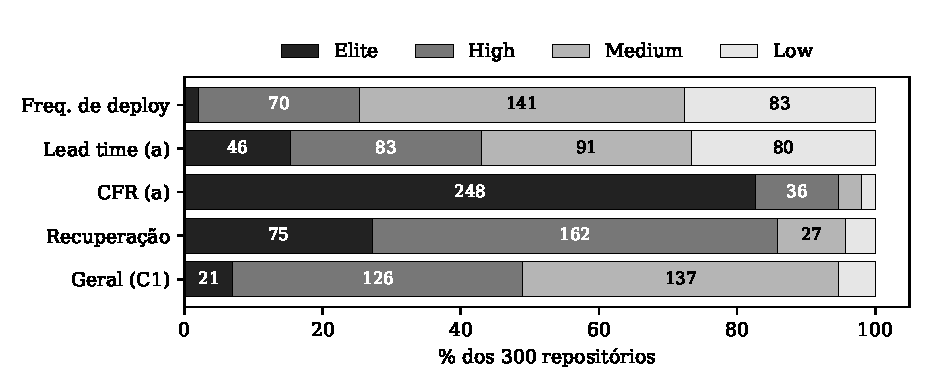
\includegraphics[width=.85\textwidth]{fig_dora_c1.pdf}
\caption{Classificação DORA de referência (C1) por dimensão}
\label{fig:dora}
\end{figure}

A Figura~\ref{fig:dora} mostra o perfil da amostra: projetos \textbf{estáveis e
lentos}. Pelo C1, 94,7\% estão em Elite ou High na taxa de falha e 85,9\% no
tempo de recuperação, mas só 25,3\% em frequência e 43,0\% em lead time.
Metade (49,0\%) fica em Elite ou High na categoria geral, puxada pelas
dimensões de estabilidade.

\subsection{RQ5: frequência de deploy e taxa de falha}

\begin{figure}[ht]
\centering
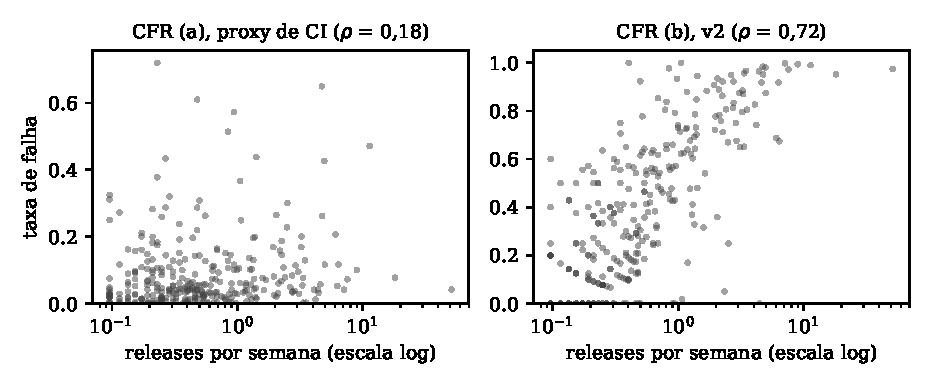
\includegraphics[width=.95\textwidth]{fig_rq05.pdf}
\caption{Frequência de deploy contra a taxa de falha, nas duas variantes}
\label{fig:rq05}
\end{figure}

Os dados \textbf{não confirmam} que velocidade e estabilidade andam juntas
(Figura~\ref{fig:rq05}). O Spearman entre releases por semana e CFR é
positivo nas duas variantes: $\rho$ = 0,178 com o CFR (a) ($p$ = 0,002) e
$\rho$ = 0,625 com o CFR (b) na variante de referência v5 ($p < 0{,}001$); nas
demais versões da heurística o valor vai de 0,635 a 0,768. Quem publica mais releases tem \emph{mais}, e não menos, falha.
O sinal é positivo em todas as combinações de definições da RQ7, mas a força
varia de fraca (0,18) a forte (0,7) conforme o CFR.

\subsection{RQ6: características associadas ao desempenho}

Dos 40 testes (4 fatores contra 10 métricas), 12 permanecem significativos
depois da correção de Holm (Tabela~\ref{tab:rq6}). Estrelas e tempo de
recuperação não mostram efeito, e nenhum fator se associa ao CFR (a).

\begin{table}[ht]
\centering
\caption{Testes significativos após Holm (Kruskal-Wallis, $n$ = 300)}
\label{tab:rq6}
\small
\begin{tabular}{lllr}
\toprule
Fator & Métrica & $p$ (Holm) & $\varepsilon^2$ \\
\midrule
Idade & Frequência de deploy & $< 0{,}001$ & 0,09 \\
Idade & Lead time (a) / (b) & $< 0{,}001$ & 0,26 / 0,19 \\
Idade & CFR (b), v1 a v5 & $\le 0{,}003$ & 0,07 a 0,18 \\
Contribuidores & Lead time (a) / (b) & $< 0{,}001$ & 0,18 / 0,16 \\
Linguagem & Lead time (a) / (b) & $< 0{,}001$ / 0,005 & 0,12 / 0,10 \\
\bottomrule
\end{tabular}
\end{table}

A \textbf{idade} é o fator mais associado. Entre o primeiro e o último
quartil de idade, a mediana de releases por semana cai de 0,81 para 0,31, o
lead time (a) sobe de 62 h para 713 h e o CFR (b) (v4) cai de 0,65 para 0,25.
Mais \textbf{contribuidores}, maior o lead time (105 h no primeiro quartil
contra 818 h no último). Quanto à \textbf{linguagem}, Java (mediana de 1.951 h),
C\# (840 h) e C++ (787 h) têm lead time bem maior que TypeScript (136 h) e
JavaScript (112 h), embora com poucos repositórios nesses grupos.

\subsection{RQ7: sensibilidade à definição operacional}

Comparamos cinco combinações: C1 (referência: release, lead time (a), CFR
(a)); C2 (release mais pré-release, lead time (b), CFR (b) na variante v5);
C3 (só o lead time muda); C4 (só o CFR muda, para a v5); e C5 (só a unidade de
deploy muda).

\begin{table}[ht]
\centering
\caption{Concordância na categoria geral entre combinações}
\label{tab:rq7}
\small
\begin{tabular}{lrrl}
\toprule
Par & \% que mudou & Kappa linear & IC 95\% \\
\midrule
C1 $\times$ C2 (tudo muda) & 34,3 & 0,496 & 0,414 -- 0,574 \\
C1 $\times$ C3 (lead time) & 19,3 & 0,732 & 0,669 -- 0,800 \\
C1 $\times$ C4 (CFR) & 23,3 & 0,660 & 0,591 -- 0,726 \\
C1 $\times$ C5 (unidade de deploy) & 1,0 & 0,986 & 0,971 -- 1,000 \\
\bottomrule
\end{tabular}
\end{table}

Entre a referência e a troca completa, cerca de 1 em cada 3 repositórios muda
de categoria (Tabela~\ref{tab:rq7}), quase sempre para pior (24,7\% descem e
9,7\% sobem). A unidade de deploy quase não importa. O lead time importa de
forma moderada (43,3\% mudam de categoria na métrica, nos dois sentidos). O
\textbf{CFR domina}: entre (a) e (b) o kappa por métrica é 0,008, isto é, não há
concordância além do acaso, e 62,0\% dos repositórios mudam de categoria nessa
dimensão. Dentro do CFR (b), a versão da heurística também pesa: a v3 muda
apenas 15,3\% dos repositórios, contra 23,3\% da v5 de referência e 34,0\% da
v4. As conclusões das RQ1 e RQ5 são, portanto, robustas no sinal, a das RQ2 é
parcial, e a da RQ3 \emph{depende totalmente} da definição.

\subsection{Validação da heurística}

\begin{table}[ht]
\centering
\caption{Concordância entre avaliadores e desempenho da heurística}
\label{tab:val}
\small
\begin{tabular}{lrr}
\toprule
Dimensão & Itens & Kappa de Fleiss \\
\midrule
Tipo do projeto & 60 & 0,920 (quase perfeita) \\
Releases são entregas reais & 60 & 0,295 (razoável) \\
Release corretiva & 300 & 0,324 (razoável) \\
\bottomrule
\end{tabular}

\vspace{6pt}
\begin{tabular}{lrrr}
\toprule
Versão & Precisão & Recall & F1 \\
\midrule
v1 \emph{patch} & 0,55 & 0,90 & 0,68 \\
v2 \emph{patch} ou nome & 0,55 & 0,90 & 0,68 \\
v3 commits & 0,69 & 0,45 & 0,54 \\
v4 combinada & 0,52 & 0,94 & 0,67 \\
v5 \emph{patch} e notas & 0,76 & 0,69 & 0,72 \\
\bottomrule
\end{tabular}
\end{table}

O tipo do projeto tem concordância quase perfeita, mas as outras duas
dimensões ficam só em ``razoável'', o que indica que ``release corretiva'' e
``entrega real'' são critérios ambíguos.

A divergência não é difusa: ela vem de \textbf{um} avaliador. O kappa de Cohen
entre os outros dois é 0,86 (quase perfeita), enquanto o do avaliador
divergente contra cada um deles é 0,19 e 0,18 (leve). Ele marcou 78\% das
releases como corretivas, contra 34\% e 37\% dos demais --- um critério mais
largo, que conta como corretiva toda release que \emph{contenha} correções, em
vez de só aquelas cujo objetivo principal é corrigir um defeito recente, que é
a definição do enunciado adotada aqui.

Optou-se por \textbf{não rerrotular}: refazer os rótulos depois de ver a saída
da heurística e as respostas dos colegas quebraria a independência que dá
sentido ao kappa. A divergência fica reportada como achado e como ameaça à
validade. Como teste de robustez, o F1 da v5 foi recalculado contra os 281
itens em que pelo menos dois avaliadores concordam: 0,737, praticamente o mesmo
valor obtido contra o consenso completo.

Nenhuma das versões v1 a v4 atinge a meta de F1 $\ge$ 0,70. As baseadas em
\emph{patch} (v1, v2 e v4) têm recall alto e precisão baixa, porque tratam todo
incremento de \emph{patch} como correção, e só 55\% dessas releases são de fato
corretivas. A v3, baseada em commits, inverte o perfil. A v5 refina a v1
exigindo também que as release notes citem correção, e chega a F1 = 0,72. O
valor é \textbf{otimista}: a v5 foi escolhida olhando parte da própria amostra,
e nas 33 releases que não participaram da escolha o F1 foi 0,65. O IC de 95\%
do F1 vai de 0,63 a 0,80. Por ser a única versão a atingir a meta, a v5 é a
variante de referência adotada no CFR (b) das RQ3, RQ5 e RQ7 (combinações C2 e
C4); as versões v1 a v4 permanecem calculadas e entram como análise de
sensibilidade na RQ7 e na RQ8.

\subsection{RQ8 (bônus): \emph{rework rate}}

A \emph{rework rate} é a proporção de releases que \emph{são} corretivas. Pela
variante de referência v5 a mediana é de 43,2\% das releases, contra 23,5\% do
CFR (b); ela é maior em 58,7\% dos repositórios, porque conta correções de
qualquer prazo, enquanto o CFR (b) só conta as que vêm em até 7 dias. Nas
versões baseadas só em \emph{patch} a rework chega a dois terços das releases
(66,7\% a 71,2\%), e com a v3 cai a 14,6\%.

O contraste nas correlações é o achado mais informativo da RQ8: o CFR (b)
acompanha a frequência de releases ($\rho$ = 0,625 na v5), e a \emph{rework
rate} praticamente não acompanha ($\rho$ = 0,008 na v5; de 0,15 a 0,26 nas
demais). Como as duas medem correção e só diferem pela exigência da janela de 7
dias, isso indica que a correlação observada na RQ5 é em boa parte
\textbf{mecânica}: quem publica mais releases tem mais chance de ter uma
release seguinte dentro da janela, e não necessariamente entrega com mais
defeitos.

\section{Discussão}

\textbf{Os proxies discordam, e isso muda a conclusão.} O CFR é a métrica em
que a escolha da definição mais pesa: o mesmo repositório é ``Elite'' pelo CI e
``Medium'' pela entrega. Isso reforça a leitura de que os proxies medem
fenômenos diferentes (falha de pipeline contra correção que chegou ao usuário)
e de que resultados em categorias DORA só fazem sentido acompanhados da
definição usada.

\textbf{Hipóteses contra resultados.} Sete das oito expectativas se
confirmaram. A frequência ficou onde se esperava (RQ1), o lead time (a) de fato
superou o (b) e em um terço dos repositórios por mais do que o dobro (RQ2), os
dois proxies de falha discordaram na direção prevista (RQ3), a recuperação
ficou em horas com censura quase nula (RQ4), a troca de definição moveu uma
parcela grande da amostra com o CFR pesando mais que o lead time (RQ7), e a
\emph{rework rate} saiu maior que o CFR (b) e muito menos correlacionada com a
frequência (RQ8). Na RQ5 a suspeita de artefato mecânico não só se confirmou
como ganhou a evidência mais limpa do trabalho: $\rho$ = 0,625 para o CFR (b)
contra 0,008 para o rework, que mede a mesma coisa sem a janela de 7 dias.

A expectativa que \textbf{falhou} foi a da RQ6. Apostamos em tipo de projeto e
número de contribuidores como fatores dominantes, e quem dominou foi a
\textbf{idade}: 8 dos 12 resultados significativos envolvem idade, contra 2 de
contribuidores e 2 de linguagem. Acertamos só a parte negativa, que estrelas
não explicariam nada. A leitura mais provável é que idade funcione como fator
de confusão, e não como causa: projetos antigos acumulam branches e commits
antigos, o que alonga o lead time (a) por construção.

Vale registrar que a previsão da RQ3 sobre a heurística também se confirmou em
detalhe: o sinal de \emph{patch} isolado deu recall 0,90 e precisão 0,55, e só
a combinação com as release notes (v5) atingiu a meta de F1.

\textbf{Velocidade e estabilidade não andam juntas, mas parte disso é efeito da
definição.} O DORA afirma que as equipes de melhor desempenho vão bem nas duas
dimensões. Aqui a frequência de deploy tem correlação positiva com a taxa de
falha. Duas leituras convivem. A primeira é substantiva: projetos que publicam
muito podem mudar mais e quebrar mais. A segunda é mecânica: o CFR (b) conta a
release seguida de uma corretiva em até 7 dias, e quem publica com frequência
tem mais chance de ter a próxima release dentro desse prazo, e a heurística
conta todo \emph{patch} como correção. O rework, que mede a mesma coisa sem a
exigência dos 7 dias, praticamente não correlaciona com a frequência ($\rho$ =
0,008 contra 0,625 do CFR (b) na v5), o que favorece fortemente a leitura
mecânica. Correlação, de qualquer forma, não implica causalidade.

\textbf{Idade é o fator mais associado, e é também um fator de confusão.}
Projetos mais novos publicam mais, têm lead time menor e mais releases
corretivas. Projetos antigos publicam menos e acumulam commits antigos, o que
alonga o lead time (a), que usa o commit mais antigo da release.

\textbf{O critério de ``corretiva'' é ambíguo.} O kappa de 0,32 e a
divergência de um avaliador mostram que a própria definição precisa de
refinamento antes de ser automatizada. Isso limita o F1 alcançável.

\section{Ameaças à validade}

\textbf{Construto.} Release publicada não é deploy, e CI vermelho não é falha em
produção: o segundo proxy subestima sistematicamente a instabilidade. A data
\texttt{author\_date} é distorcida por \emph{rebase} e \emph{squash merge}, e
commits com data posterior à release contam como 0 h. A heurística corretiva
tem erro relevante: nenhuma versão v1 a v4 atinge F1 de 0,70, a v5 foi escolhida
na própria amostra, e o CFR (b) pode estar correlacionado com a frequência de
deploy por construção. Tags não foram usadas como unidade de deploy.

\textbf{Interna.} Repositórios mais antigos acumulam mais releases e commits
antigos, e a idade se associa a várias métricas (RQ6). O tipo do projeto, que
seria um quinto fator, não entrou na análise.

\textbf{Externa.} A amostra tem projetos populares, com GitHub Actions e
releases regulares. Ela não representa projetos privados nem os que publicam
sem releases do GitHub. A janela é de 12 meses.

\textbf{Conclusão.} Foram 36 testes no RQ6, corrigidos por Holm, e alguns
grupos têm poucos repositórios (linguagens raras). A amostra-ouro tem 300
releases de 60 repositórios, e o kappa em duas dimensões é apenas razoável. A
censura foi tratada, mas episódios de falha sem recuperação reduzem o tempo de
recuperação medido.

\section{Replicação cruzada}

[PREENCHER na entrega final: qual pipeline foi replicado, se foi possível
executá-lo só pelo README, diferença relativa por métrica e \% de repositórios
com a mesma classificação DORA em relação ao CSV original, e as issues abertas
e recebidas.]

\section{Conclusão}

Medimos as métricas DORA em 300 repositórios populares e mostramos que o valor
da métrica depende mais da definição operacional do que se poderia esperar. A
taxa de falha varia por um fator de cinco entre os dois proxies, e 34,3\%
dos repositórios mudam de categoria quando as definições mudam. A frequência de
deploy não se associa a menos falhas, e a idade é o fator mais ligado ao
desempenho. A validação manual mostrou que a classificação de release
corretiva é ambígua, e mesmo a heurística de referência (v5) atinge F1 de
apenas 0,72. Como trabalho futuro, propomos refinar o critério de ``release
corretiva'' com mais avaliadores e com um protocolo de rotulagem mais
explícito, e usar tags como unidade de deploy. O código, os dados e os resultados estão em
\url{https://github.com/gabrielchagas13/lab-exp-de-software-turma-02-grupo-06},
e o processo do grupo (GitHub Projects) em
\url{https://github.com/gabrielchagas13/lab-exp-de-software-turma-02-grupo-06/projects}.

\bibliographystyle{sbc}
\bibliography{sbc-template}

\end{document}
